\documentclass{article}
\usepackage[utf8]{inputenc}
\usepackage{tabularx} % extra features for tabular environment
\usepackage{amsmath}  % improve math presentation
\usepackage{graphicx} % takes care of graphic including machinery
\usepackage{xspace}
\usepackage{tikz}
\usepackage{enumitem}
\usetikzlibrary{babel}
\usepackage[american]{circuitikz}
\usetikzlibrary{calc}
\usepackage{listings}
\usepackage{float}
\usepackage{siunitx}
\usepackage{pgfplots}
\usepackage[skins,theorems]{tcolorbox}
\tcbset{highlight math style={enhanced,
  colframe=red,colback=white,arc=0pt,boxrule=1pt}}
\pgfplotsset{width=10cm,compat=1.9}
\usepackage[margin=1in,letterpaper]{geometry} % decreases margins
\usepackage{cite} % takes care of citations
\usepackage[final]{hyperref} % adds hyper links inside the generated PDF file
\hypersetup{
colorlinks=true,       % false: boxed links; true: colored links
linkcolor=blue,        % color of internal links
citecolor=blue,        % color of links to bibliography
filecolor=magenta,     % color of file links
urlcolor=blue        
}

\begin{document}

\title{{\textbf{MINI PROJECT 2}}}
\author{\textbf{TADIPATRI UDAY KIRAN REDDY}\\\textbf{EE19BTECH11038}}
\maketitle

\section*{\hfil Justification}
\begin{figure}[H]
	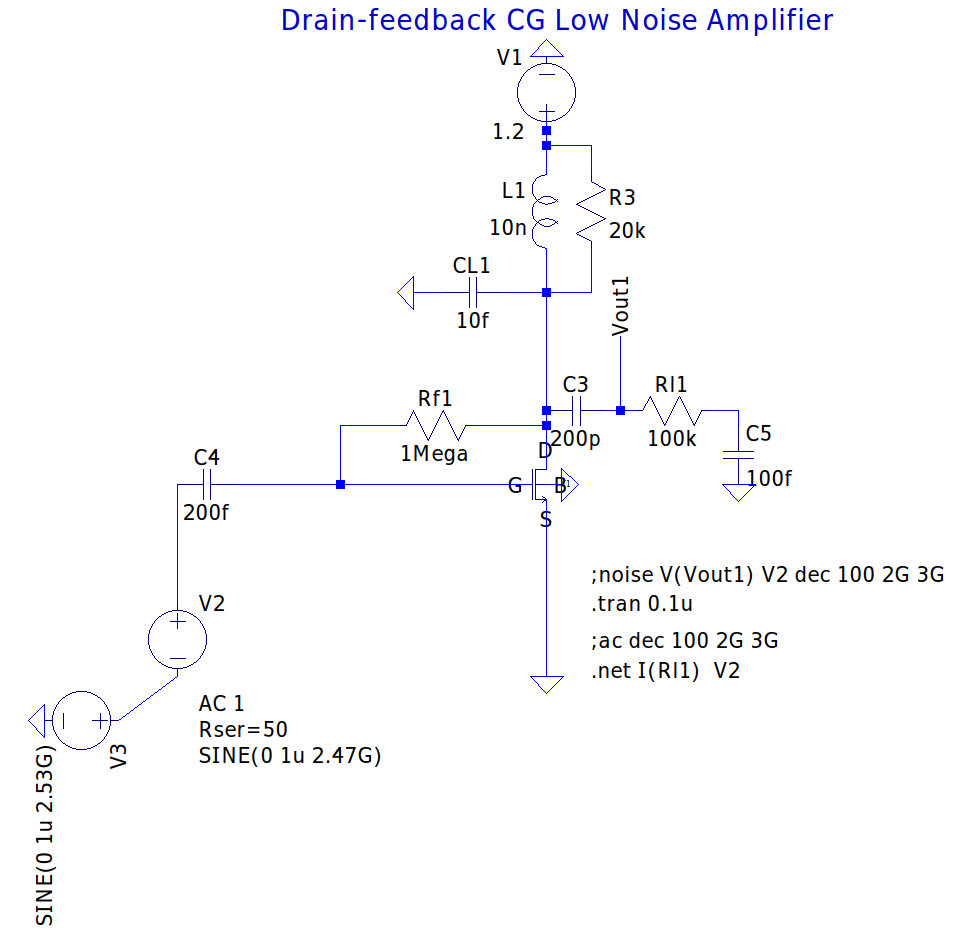
\includegraphics[scale=0.4]{../figs/sch.png}
\end{figure}
\begin{itemize}
	\item This implementation is Drain-feedback Common Gain Noise Low Noise Amplifier with inductor degeneration.
	\item The drain feedback ensures DC biasing.
	\item Inductor ensures that low pass gain is pushed to bandpass in our desired frequency range of  2GHz-3GHz.
	\item $Nf = 1 + \frac{R_s}{R_f} + \frac{\gamma}{g_mR_s} + \frac{1}{R_sR_dg_m^2}$, High drain feedback and high transconductance ensure low Noise figures.
\end{itemize}
\section*{\hfil Design specifications}
NMOS of L=65nm and W=100$\mu$m is used.
\subsection*{Netlist}
\begin{lstlisting}
* Z:\home\solomon\ICWC\Mini_Projects\Mini_Project_2\final_lna.asc
XX1 N004 N002 0 0 nmos65 params: L=65nm, W=100um, M=10
V1 N001 0 1.2
C3 Vout1 N002 200p
Rl1 N003 Vout1 100k
C4 N004 N005 200f
Rf1 N002 N004 1Mega
L1 N002 N001 10n Rser=1.57k
CL1 N002 0 10f
C5 N003 0 100f
V2 N005 N006 SINE(0 1u 2.47G) AC 1 Rser=50
R3 N001 N002 20k
V3 N006 0 SINE(0 1u 2.53G)

* block symbol definitions
.subckt nmos65 G D S B
M1 D G S B NMOS l={L} w={W} ad='2*65n*{W}' as='2*65n*{W}' pd='2*(2*65n+{W})' ps='2*(2*65n+{W})' m={M}
.PARAM L=65n W=1u M=1
.ends nmos65

.model NMOS NMOS
.model PMOS PMOS
.lib C:\users\solomon\My Documents\LTspiceXVII\lib\cmp\standard.mos
;ac dec 100 2G 3G
.tran 0.1u
;noise V(Vout1) V2 dec 100 2G 3G
.net I(Rl1)  V2
* Drain-feedback CG Low Noise Amplifier
.backanno
.end
\end{lstlisting}
\subsection*{Gain}
\begin{figure}[H]
	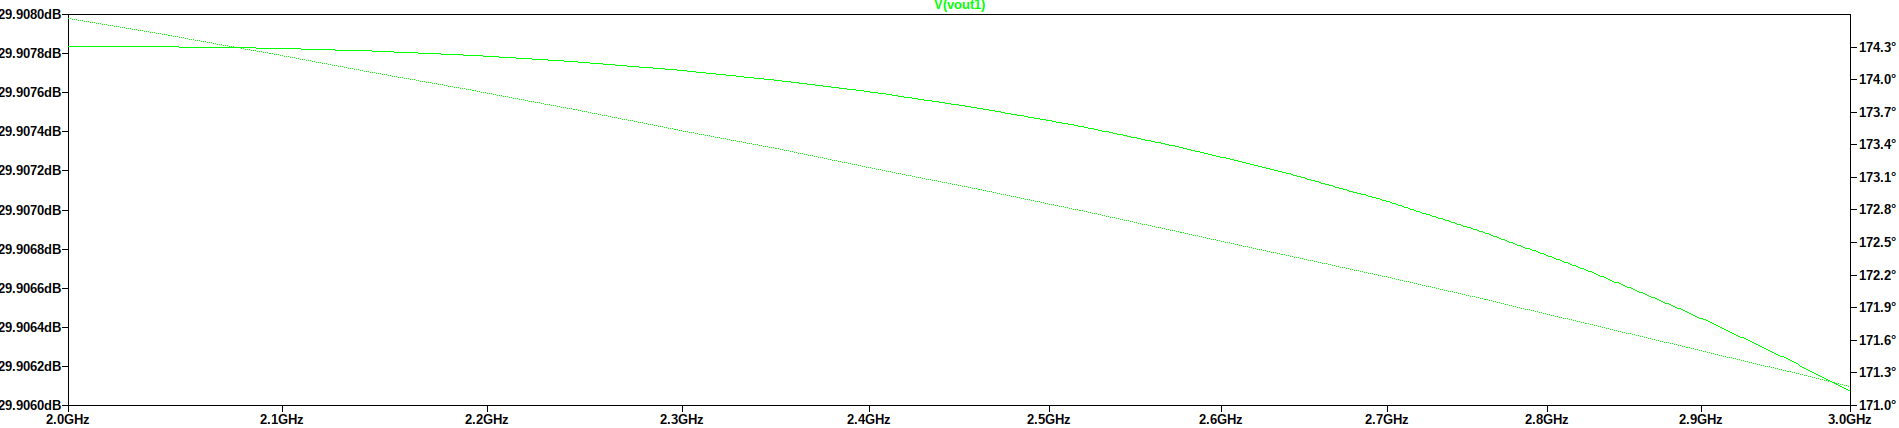
\includegraphics[scale=0.27]{../figs/gain.png}
\end{figure}
A gain of \textbf{29.9dB} was obtained.
\subsection*{Noise Figure}
\begin{figure}[H]
	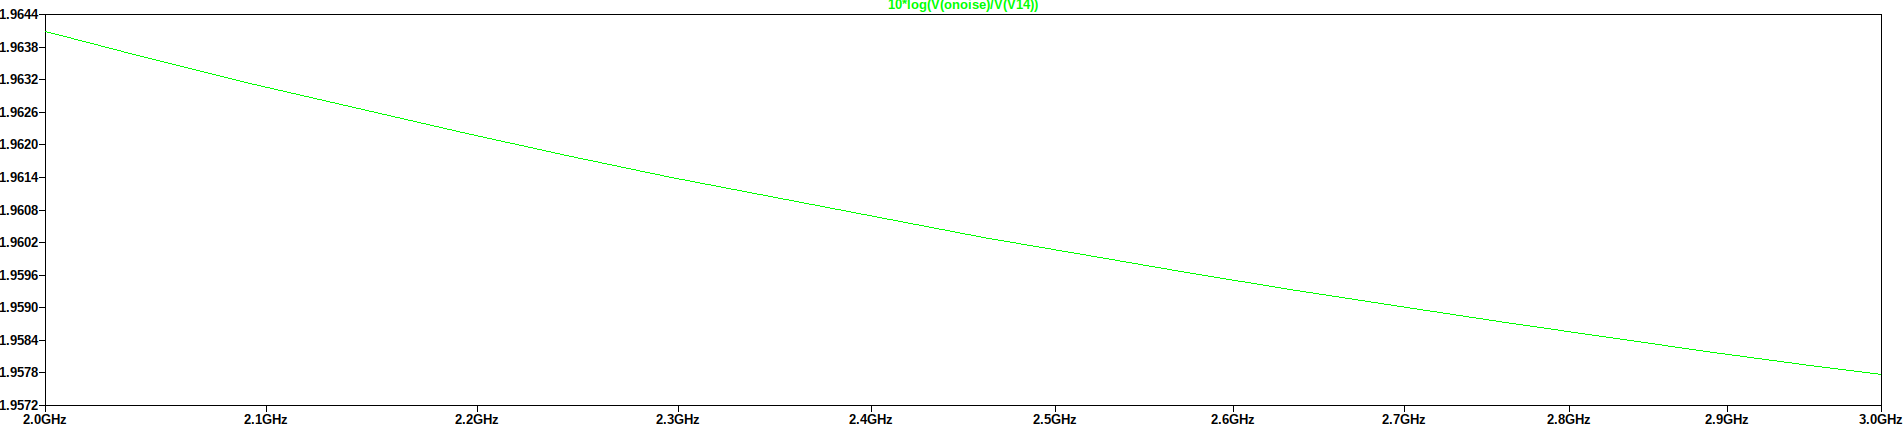
\includegraphics[scale=0.27]{../figs/nf.png}
\end{figure}
Noise figure is below \textbf{1.96dBm}.
\subsection*{Input Return Loss}
\begin{figure}[H]
	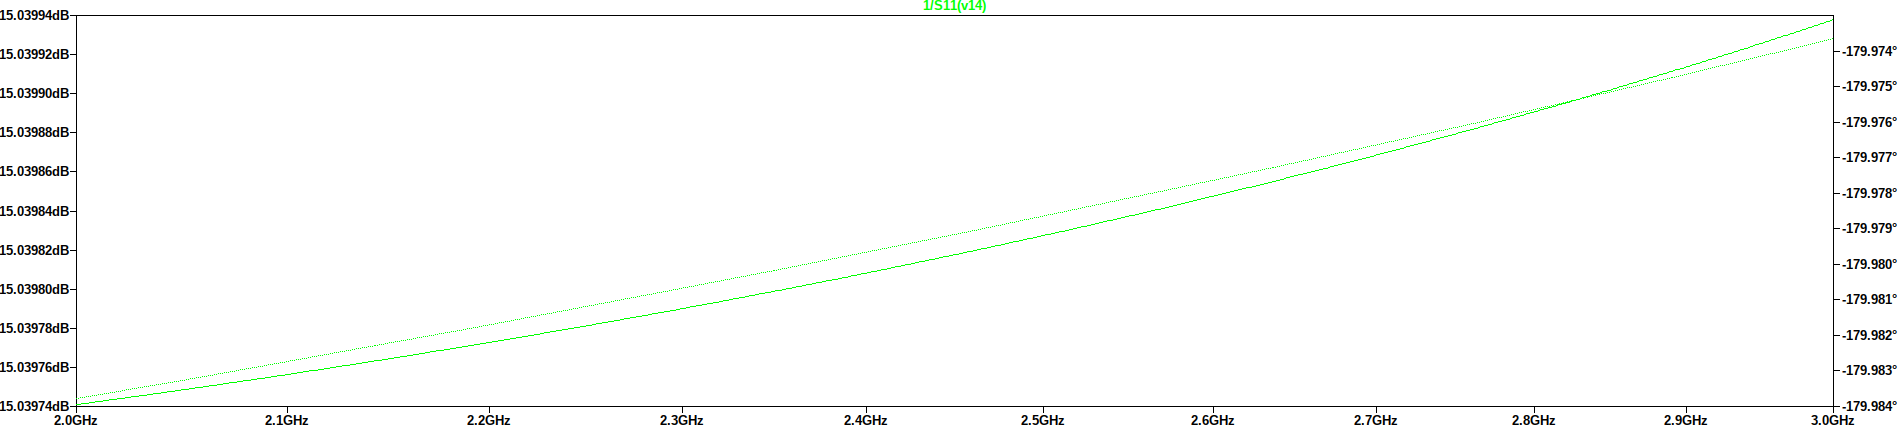
\includegraphics[scale=0.27]{../figs/Input_returnloss.png}
\end{figure}
Input return loss is \textbf{15dB}.
\subsection*{Dual-tone test}
\begin{figure}[H]
	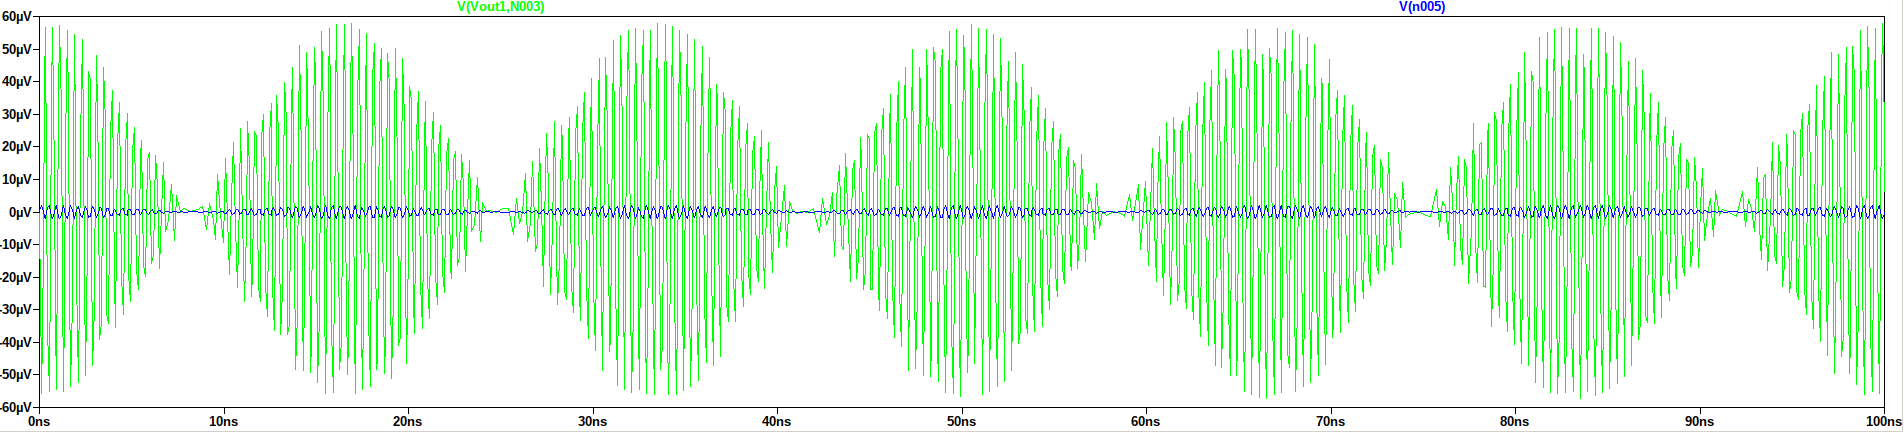
\includegraphics[scale=0.27]{../figs/2tone.png}
\end{figure}
Input signal consists of two sinusoids at 2.47GHz and 2.53GHz.
\begin{figure}[H]
	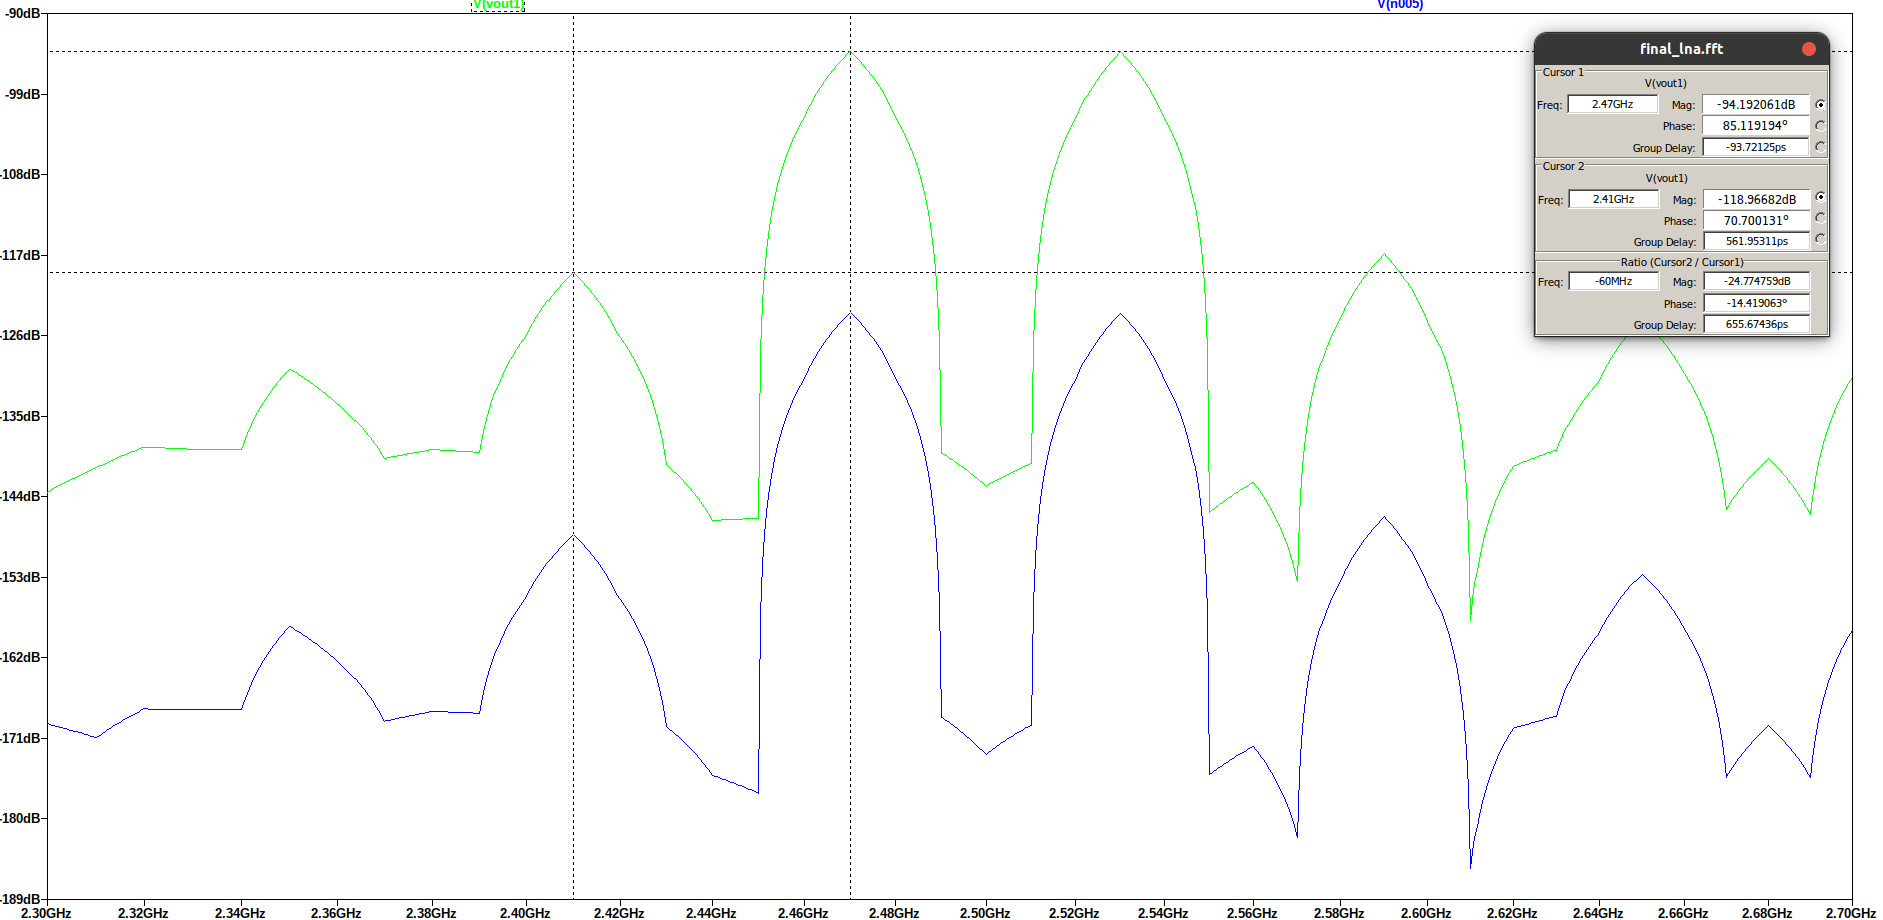
\includegraphics[scale=0.27]{../figs/2tone_ft.png}
\end{figure}

\begin{gather*}
	A_1 = -94.2dB; A_2 = -118.97dB\\
	IIP_3 = \frac{\Delta P}{2} + P_{in}\\
	\mathbf{IIP_3 = -47.6dB}
\end{gather*}
\section*{\hfil Obtained specifications}
\begin{itemize}
	\item \textbf{Gain} = 29.9dB
	\item \textbf{Input return loss} = 15dB
	\item  \textbf{Noise figure} = 1.96dBm
	\item \textbf{IIP3} = -47.6dB
\end{itemize}
\end{document}